% !TeX spellcheck = pl_PL
\begin{appendices}
 	\chapter{Przykład serializacji}\label{add:A}
 	\begin{center}
 		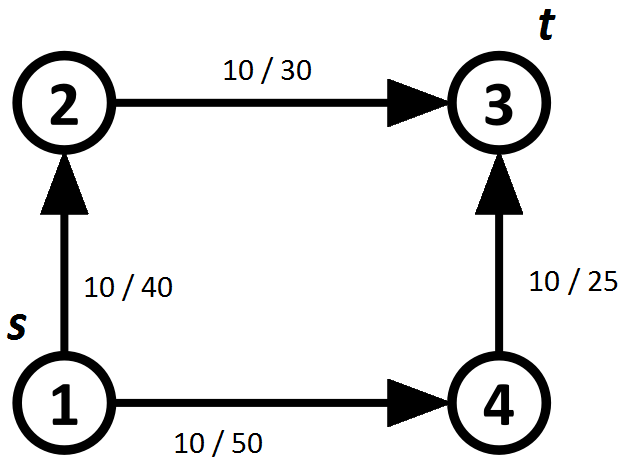
\includegraphics[width=0.5\textwidth]{./img/serialized_graph.png}
 	\end{center}
 	\lstinputlisting[language=xml,basicstyle=\small\label{key}\ttfamily]{./listings/serialized_graph.xml}
 	\vfill
 	\lstinputlisting[language=xml,basicstyle=\small\label{key}\ttfamily,firstnumber=22]{./listings/serialized_graph_model.xml}
 	\vfill
 	\chapter{Tworzenie sieci residualnej}\label{add:B}
 	\vspace{-1cm}
 	\cppcode{./listings/makeResidualNetwork.cpp}
 	\chapter{Szukanie ścieżki w sieci}
 	\cppcode{./listings/findPathBetween.cpp}\label{add:findPathAlg}
 	\chapter{Zwiększenie przepływu w sieci}
 	\cppcode{./listings/increaseFlow.cpp}\label{add:increaseFlowAlg}
 	\chapter{Warunki stopu}\label{add:stopConditionsAlg}
 	\cppcode{./listings/stopConditions1.cpp}
 	\cppcode{./listings/stopConditions2.cpp}\vfill
 	\cppcode{./listings/stopConditions3.cpp}
 	\chapter{Klasa algorytmu Forda-Fulkersona}\label{add:fordFulkersonAlg}
 	\cppcode{./listings/fordFulkersonAlg.cpp}
 	\chapter{Realizacja algorytmu Floyda-Warshalla}\label{add:floydWarshallImpl}
 	\cppcode{./listings/floydWarshall.cpp}
 	\chapter{Usuwanie elementów nadmiarowych z sieci residualnej}\label{add:removeRedundantElements}
 	\cppcode{./listings/removeRedundantElements.cpp}
 	\cppcode{./listings/hideRedundantVertices.cpp}\vfill
 	\cppcode{./listings/removeRedundantEdges.cpp}
 	\chapter{Zapełnianie przepływu blokującego}\label{add:blockPrzeplywZapel}
 	\vspace{-1cm}
 	\cppcode{./listings/block_findAugumentingPathInBlockingFlow.cpp}
 	\cppcode{./listings/block_pushBlockingSet.cpp}
 	\cppcode{./listings/block_increaseFlow.cpp}
 	\chapter{Algorytm MKM}\label{add:mkmImpl}
 	\vspace{-0.5cm}
 	\cppcode{./listings/mkm_findAugumentingPath.cpp}
 	\cppcode{./listings/mkm_findVertexWithMinimalPotential.cpp}
 	\chapter{Realizacja algorytmu Forda-Fulkersona}\label{add:C}
 	\setlength\intextsep{10pt}
 	\begin{figure}[H]
 		\centering
 		\begin{subfigure}{\textwidth}
 			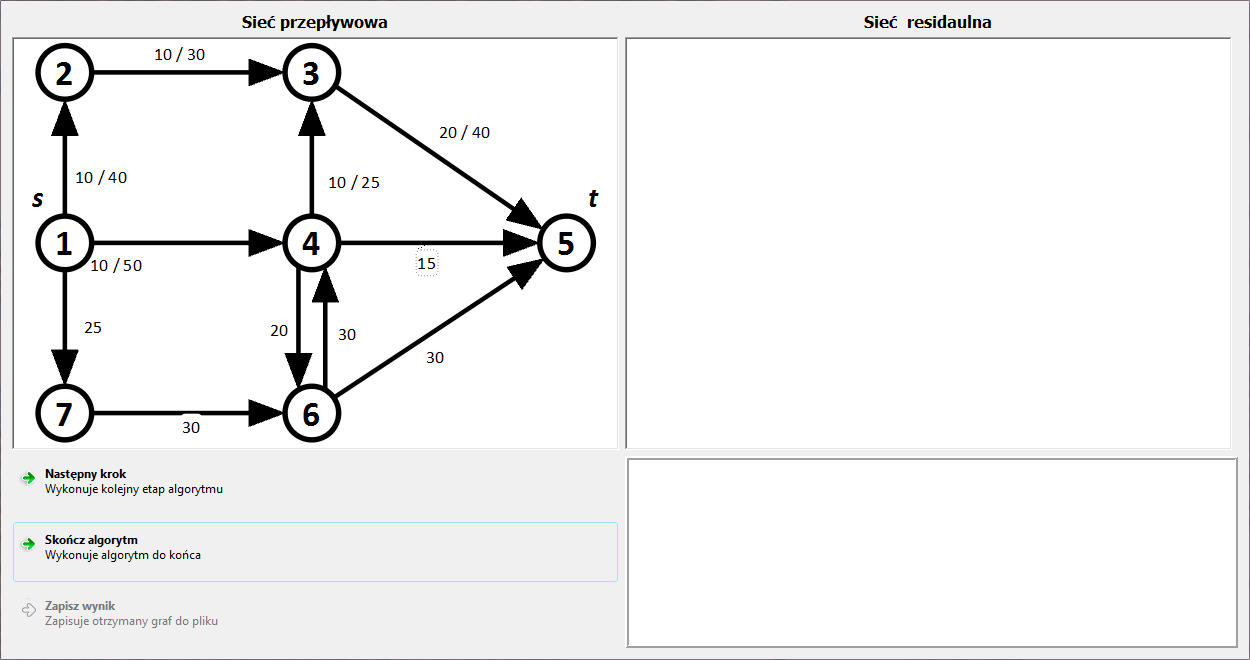
\includegraphics[width=0.9\linewidth]{./img/spec_zew06_1.png}
 		\end{subfigure}\par\bigskip
 		\begin{subfigure}{\textwidth}
 			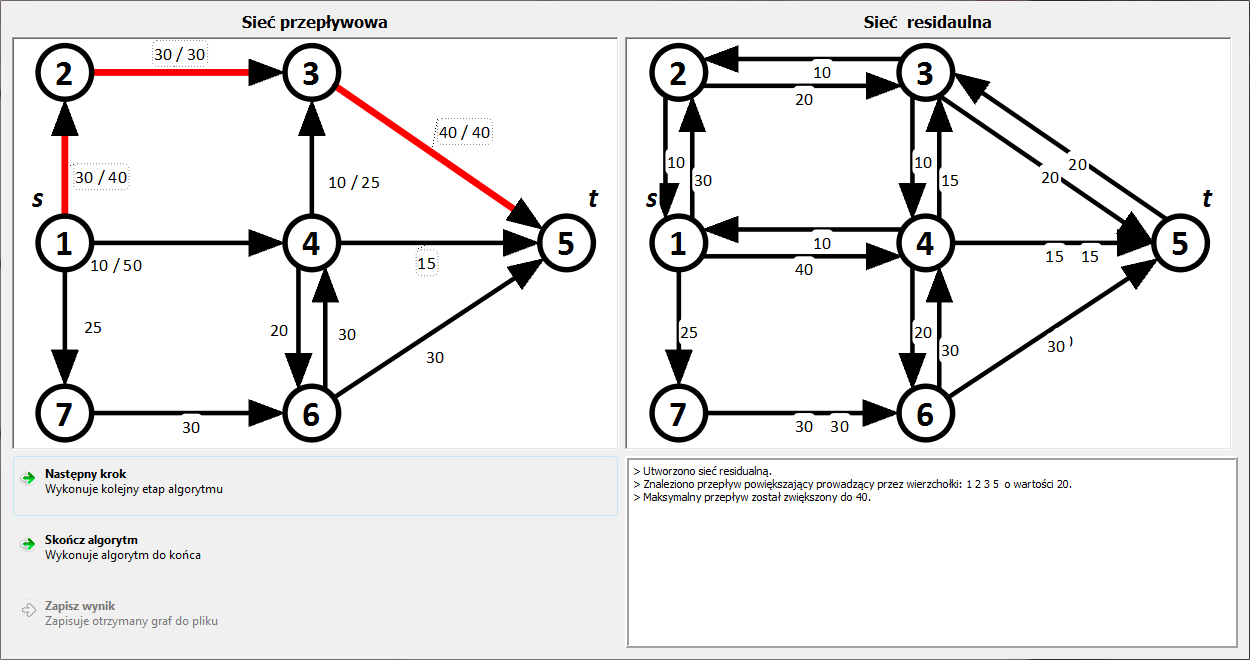
\includegraphics[width=0.9\linewidth]{./img/spec_zew06_2.png}
 		\end{subfigure}
 	\end{figure}
 	\begin{figure}[H]
 		\ContinuedFloat
 		\begin{subfigure}{\textwidth}
 			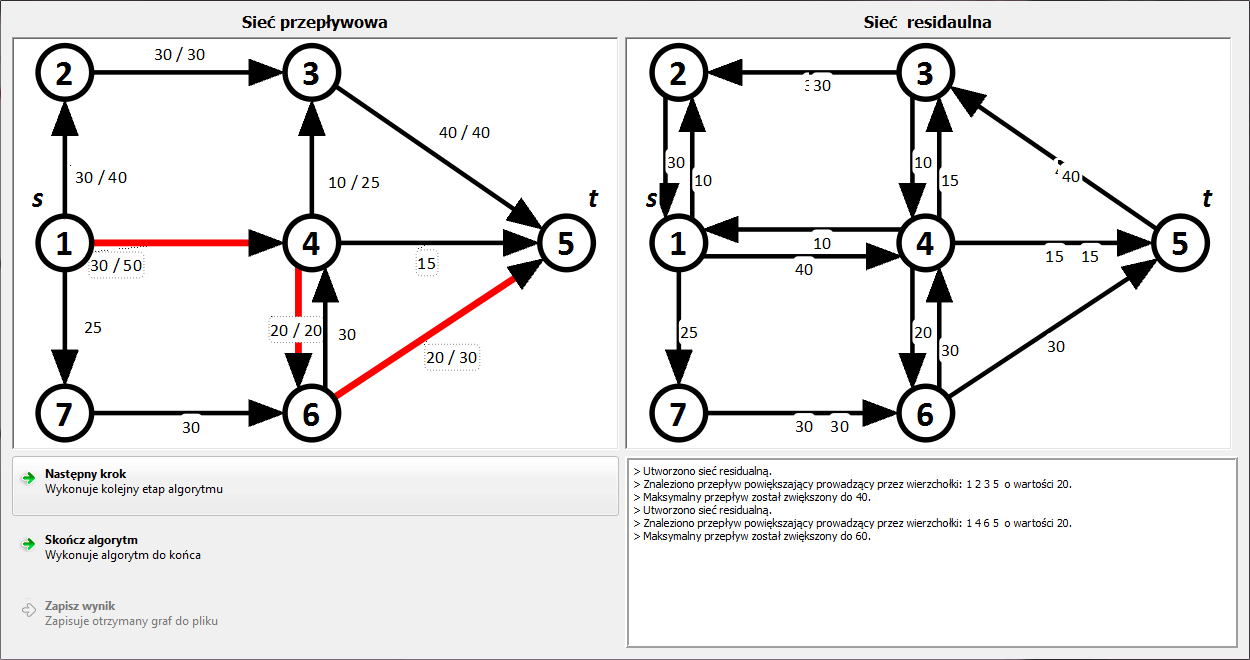
\includegraphics[width=0.9\linewidth]{./img/spec_zew06_3.png}
 		\end{subfigure}\par\bigskip
 		\begin{subfigure}{\textwidth}
 			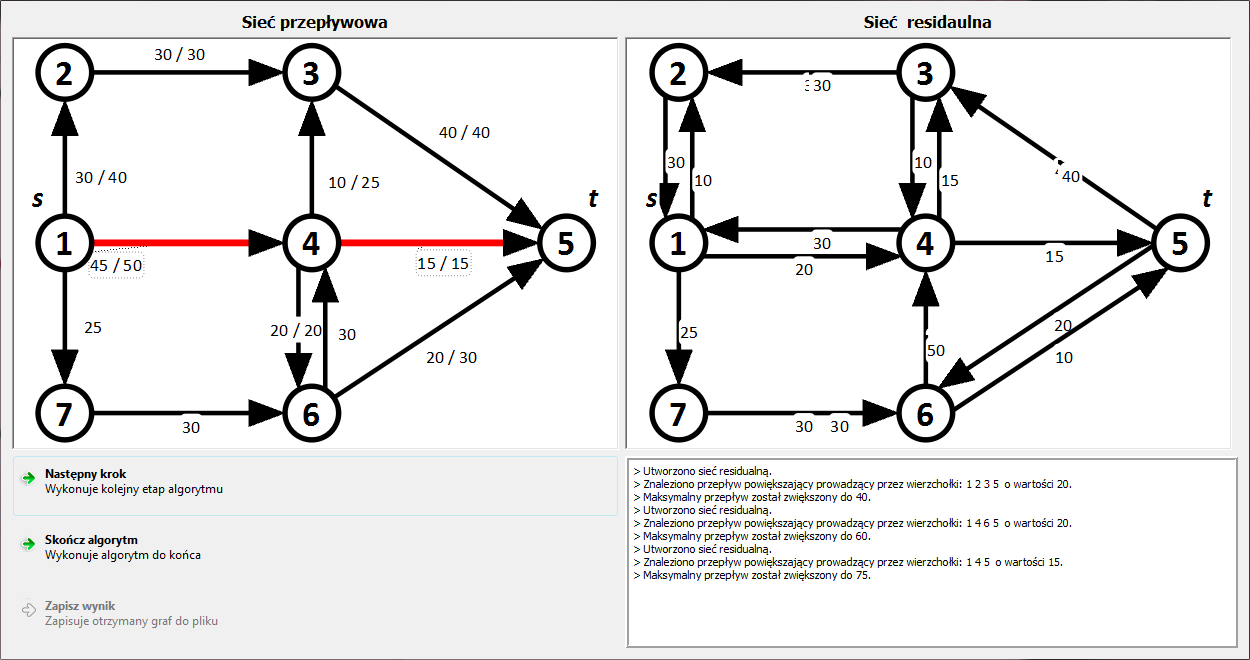
\includegraphics[width=0.9\linewidth]{./img/spec_zew06_4.png}
 		\end{subfigure}\par\bigskip
 		\begin{subfigure}{\textwidth}
 			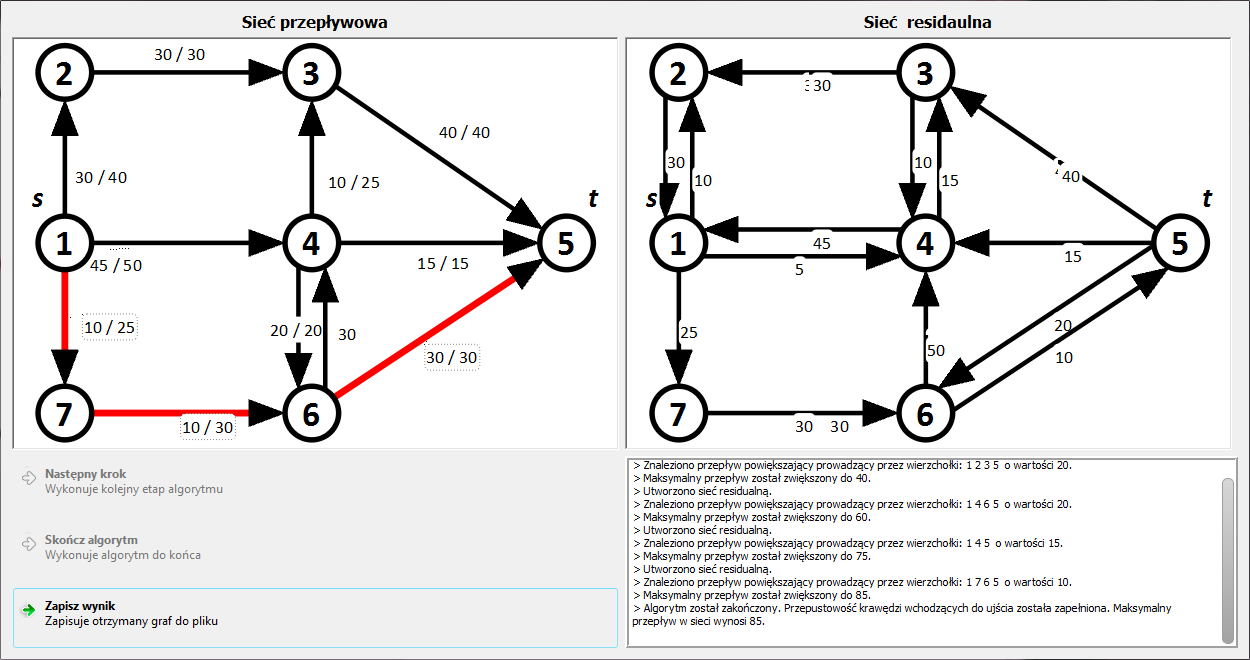
\includegraphics[width=0.9\linewidth]{./img/spec_zew06_5.png}
 		\end{subfigure}
 	\end{figure}
 	\chapter{Realizacja algorytmu Dinica}\label{add:dinicExample}
 	\setlength\intextsep{10pt}
 	\begin{figure}[H]
 		\centering
 		\begin{subfigure}{\textwidth}
 			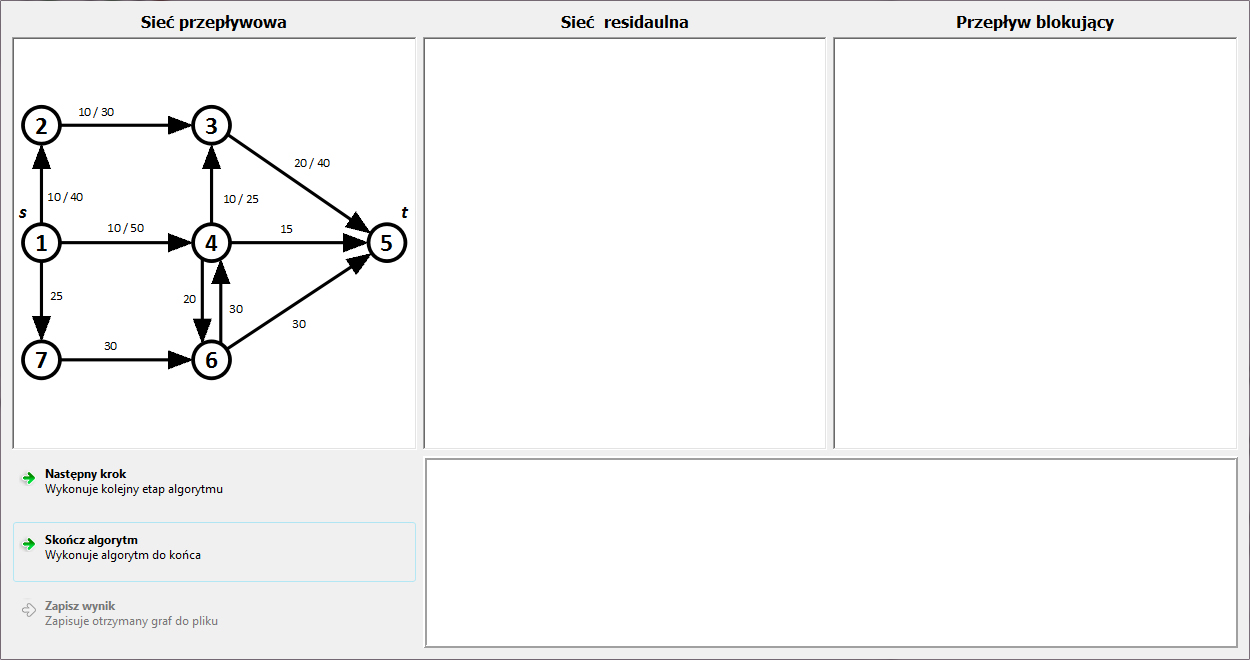
\includegraphics[width=0.9\linewidth]{./img/dinic01.jpg}
 		\end{subfigure}\par\bigskip
 		\begin{subfigure}{\textwidth}
 			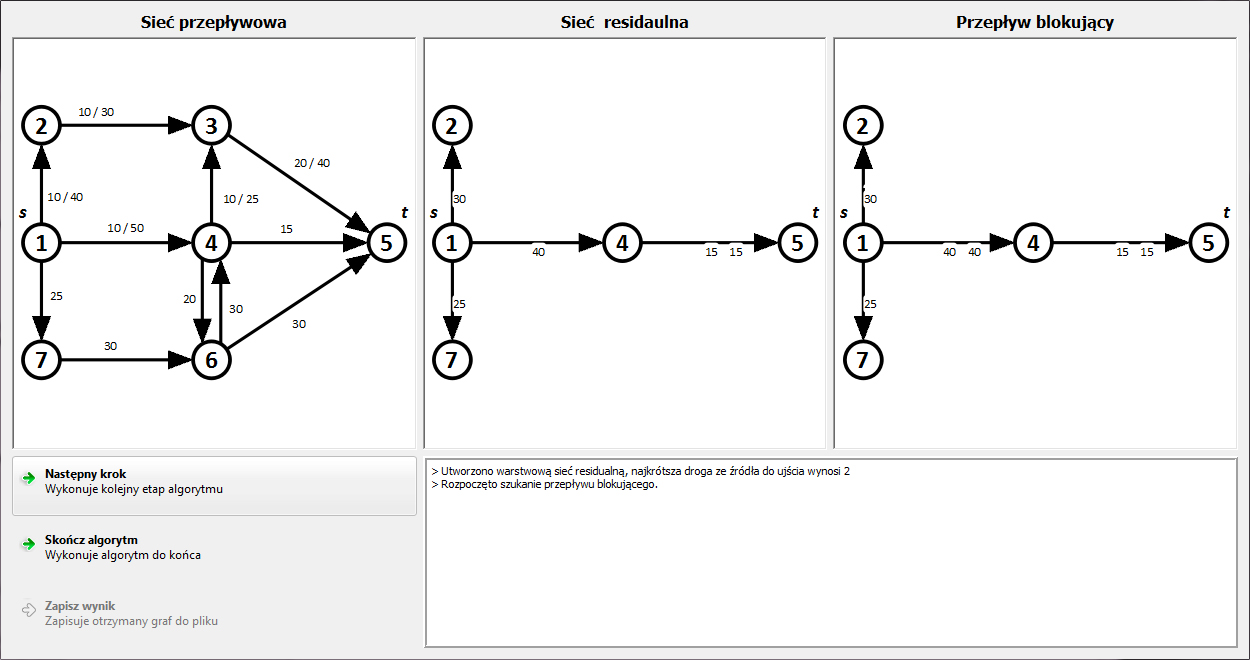
\includegraphics[width=0.9\linewidth]{./img/dinic02.jpg}
 		\end{subfigure}
 	\end{figure}
 	\begin{figure}
 		\ContinuedFloat
 		\begin{subfigure}{\textwidth}
 			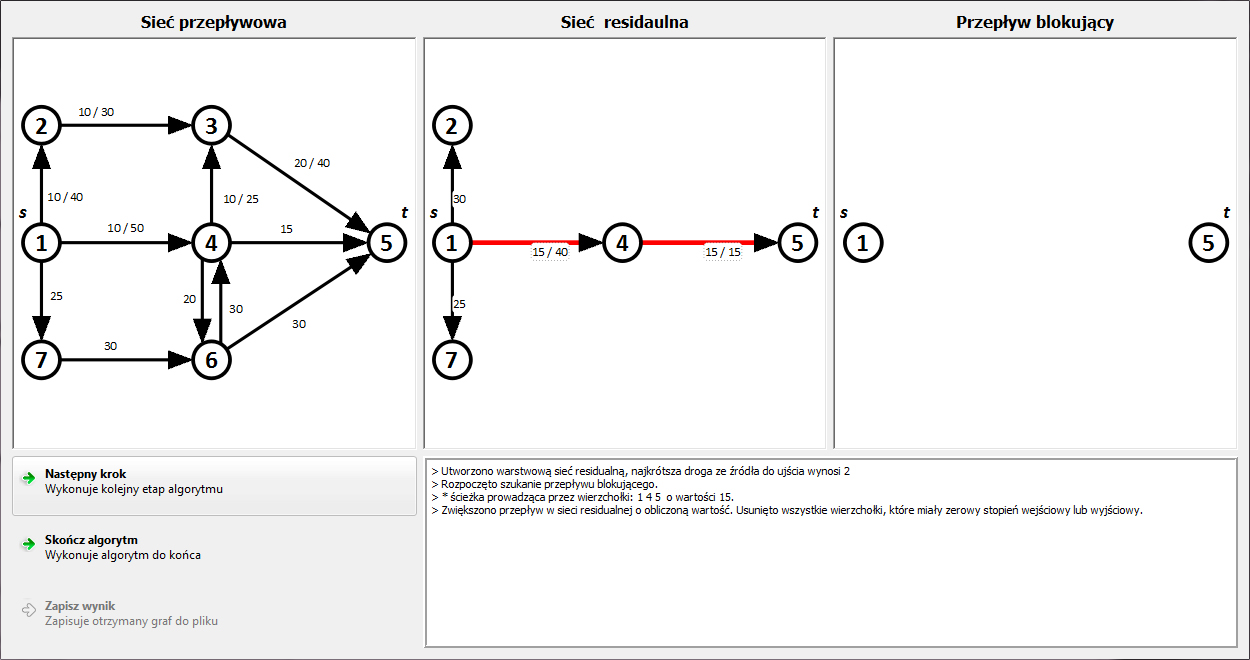
\includegraphics[width=0.9\linewidth]{./img/dinic03.jpg}
 		\end{subfigure}\par\bigskip
 		\begin{subfigure}{\textwidth}
 			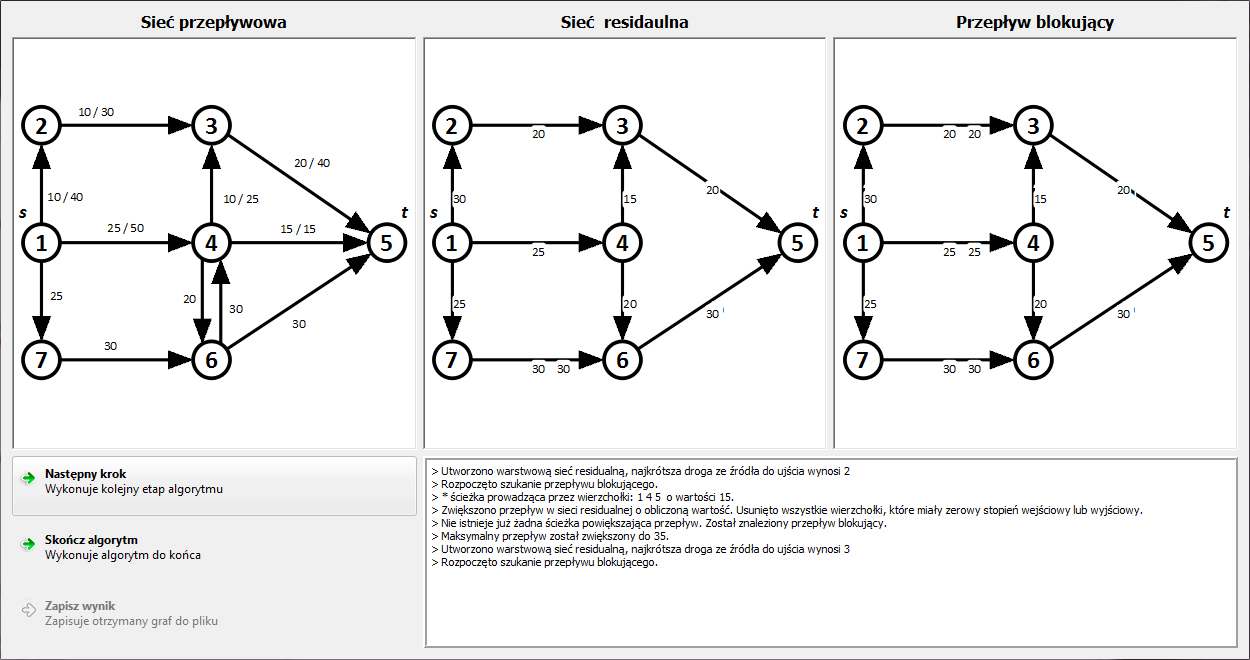
\includegraphics[width=0.9\linewidth]{./img/dinic05.jpg}
 		\end{subfigure}\par\bigskip
 		\begin{subfigure}{\textwidth}
 			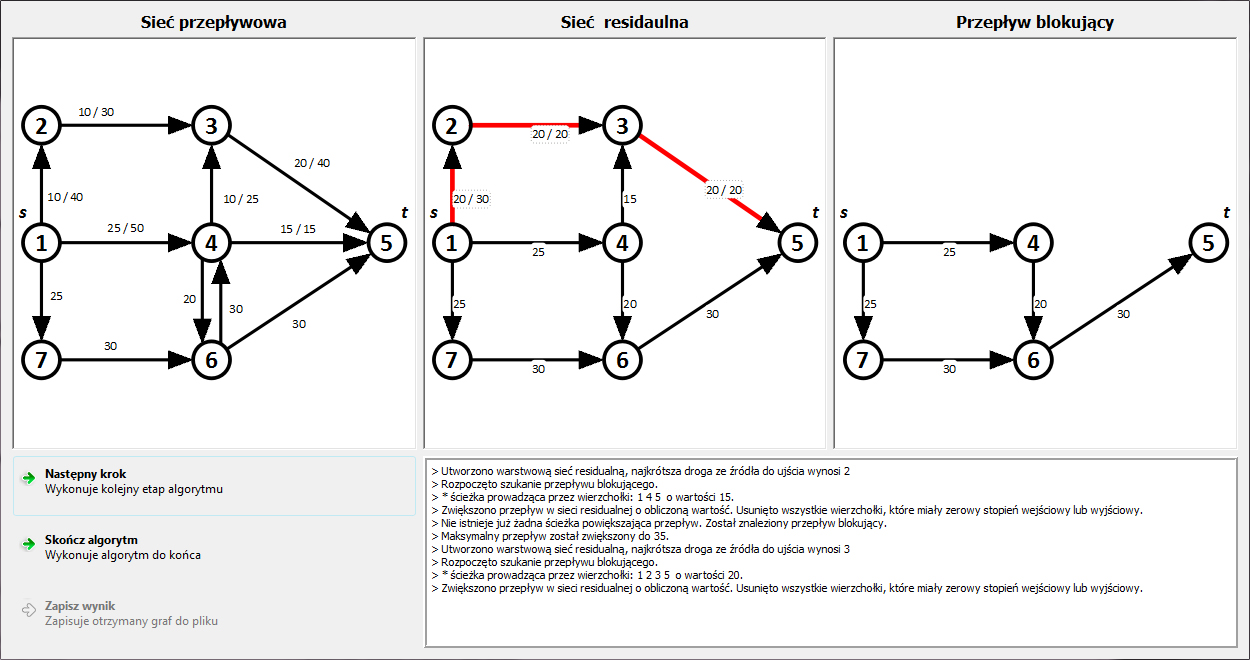
\includegraphics[width=0.9\linewidth]{./img/dinic06.jpg}
 		\end{subfigure}
 	\end{figure}
 	\begin{figure}
 		\ContinuedFloat
 		\begin{subfigure}{\textwidth}
 			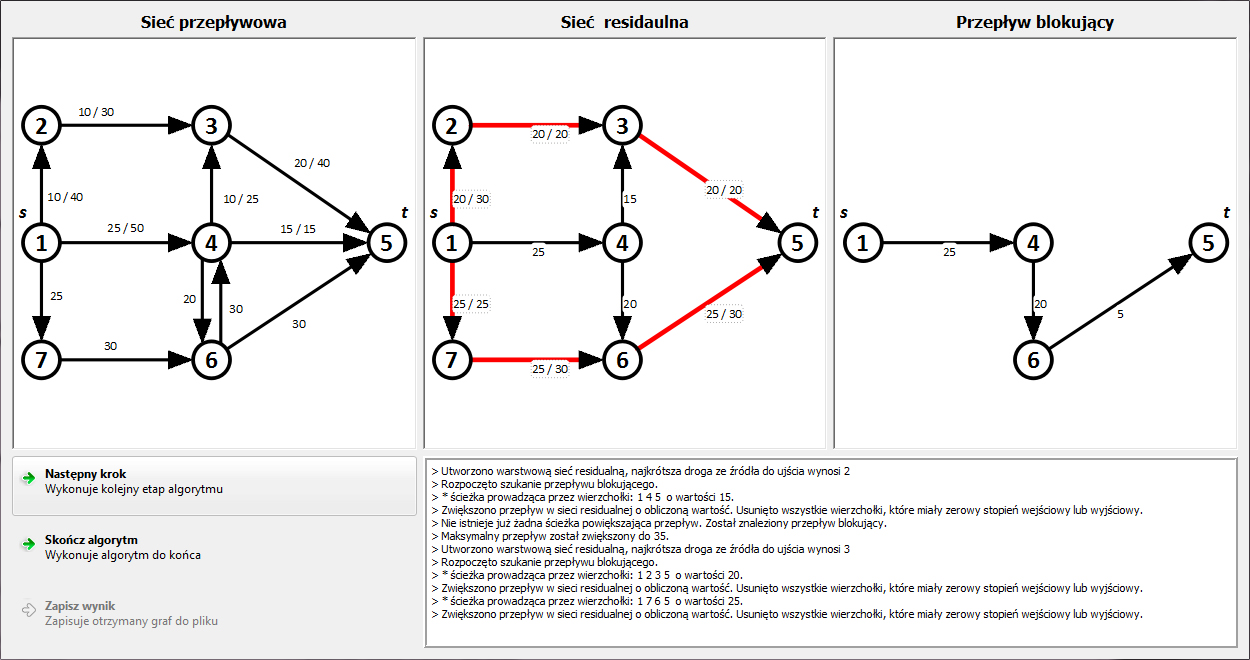
\includegraphics[width=0.9\linewidth]{./img/dinic07.jpg}
 		\end{subfigure}\par\bigskip
 		\begin{subfigure}{\textwidth}
 			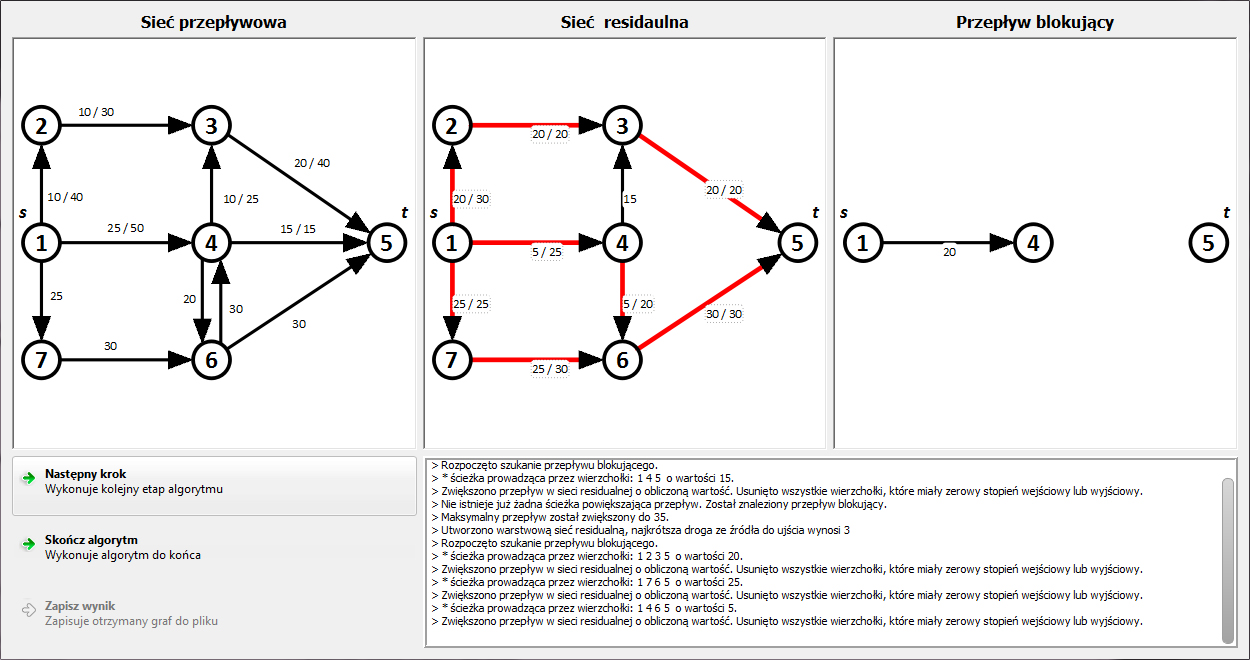
\includegraphics[width=0.9\linewidth]{./img/dinic08.jpg}
 		\end{subfigure}
 		\begin{subfigure}{\textwidth}
 			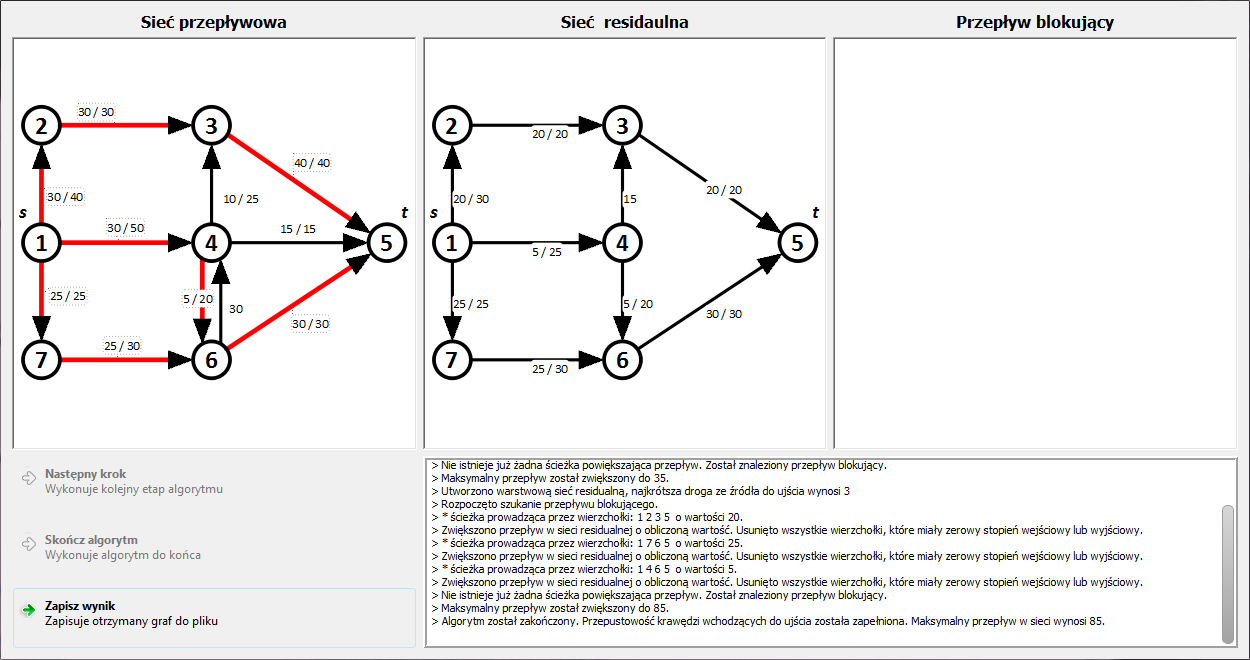
\includegraphics[width=0.9\linewidth]{./img/dinic09.jpg}
 		\end{subfigure}
 	\end{figure}
 	\chapter{Realizacja algorytmu MKM}\label{add:mkmExample}
 	\setlength\intextsep{10pt}
 	\begin{figure}[H]
 		\centering
 		\begin{subfigure}{\textwidth}
 			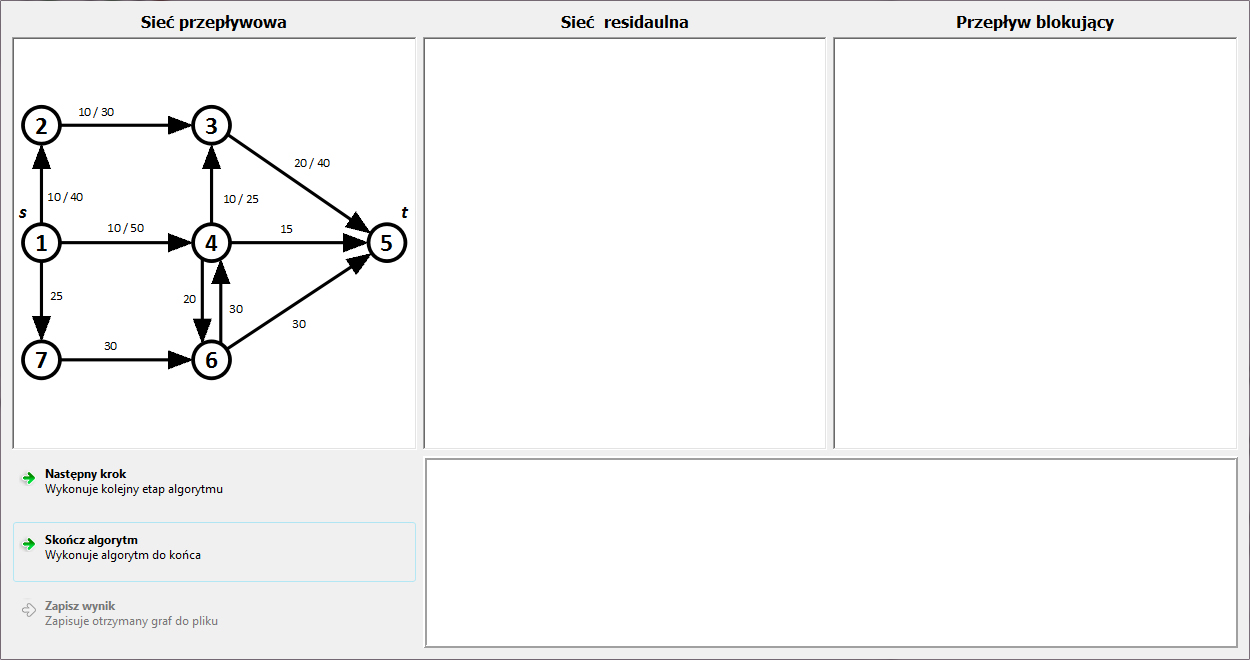
\includegraphics[width=0.9\linewidth]{./img/mkm01.jpg}
 		\end{subfigure}\par\bigskip
 		\begin{subfigure}{\textwidth}
 			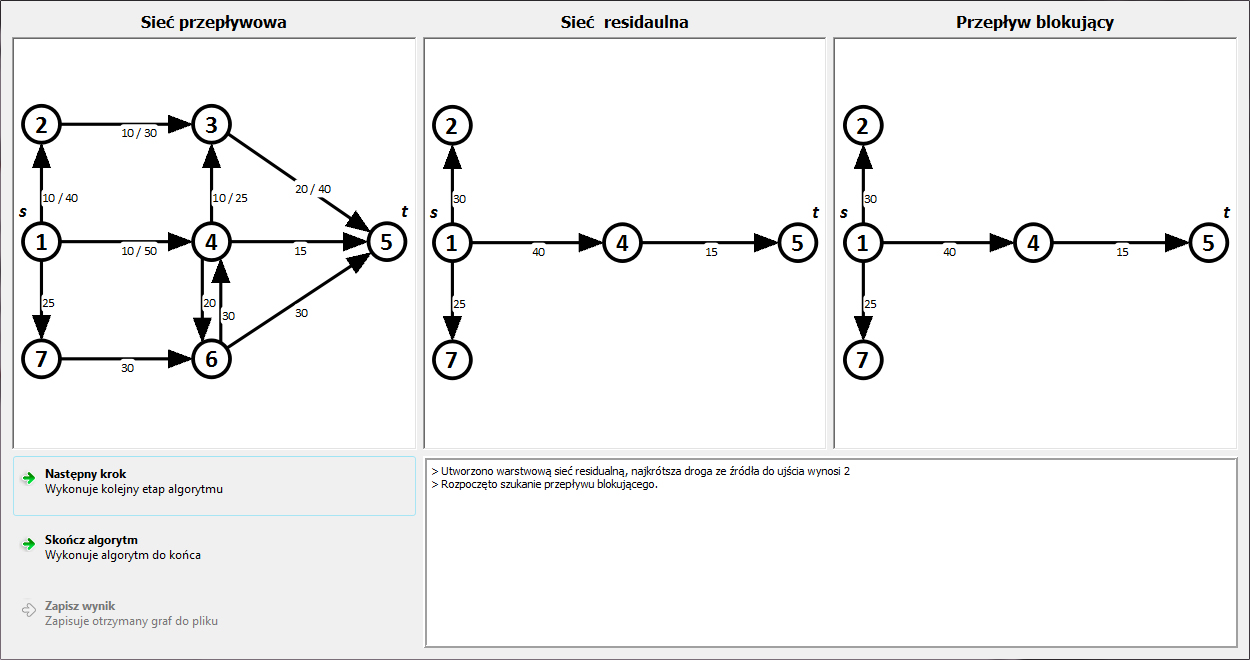
\includegraphics[width=0.9\linewidth]{./img/mkm02.jpg}
 		\end{subfigure}
 	\end{figure}
 	\begin{figure}
 		\ContinuedFloat
 		\begin{subfigure}{\textwidth}
 			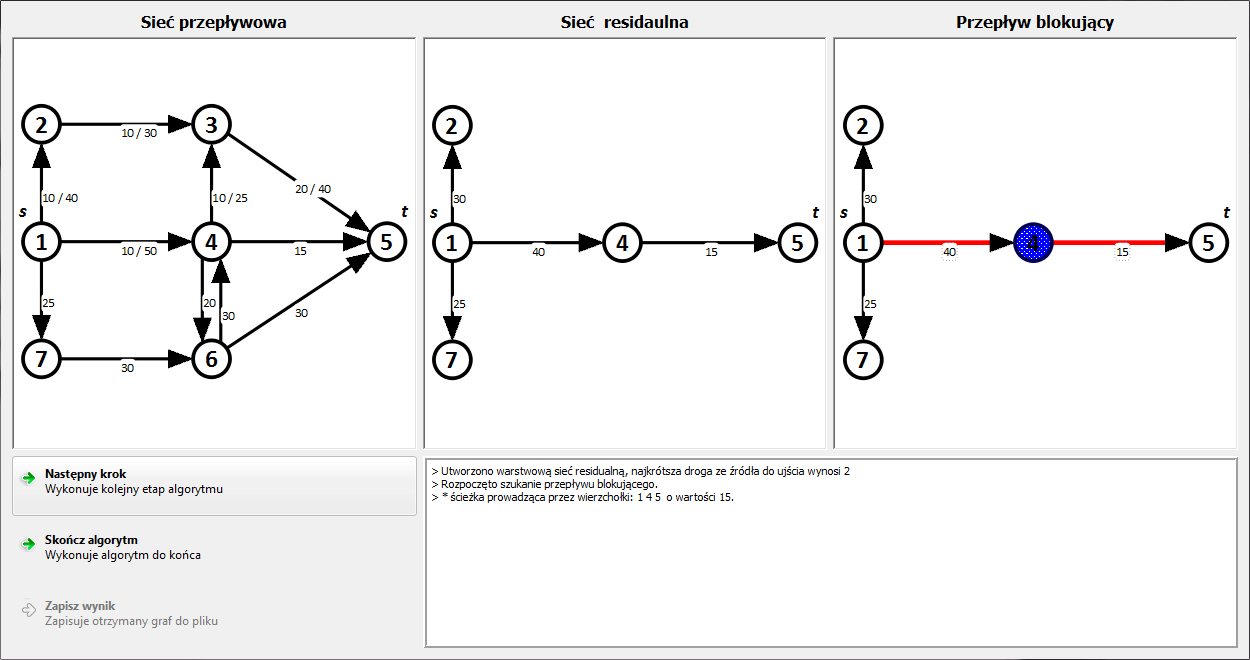
\includegraphics[width=0.9\linewidth]{./img/mkm03.jpg}
 		\end{subfigure}\par\bigskip
 		\begin{subfigure}{\textwidth}
 			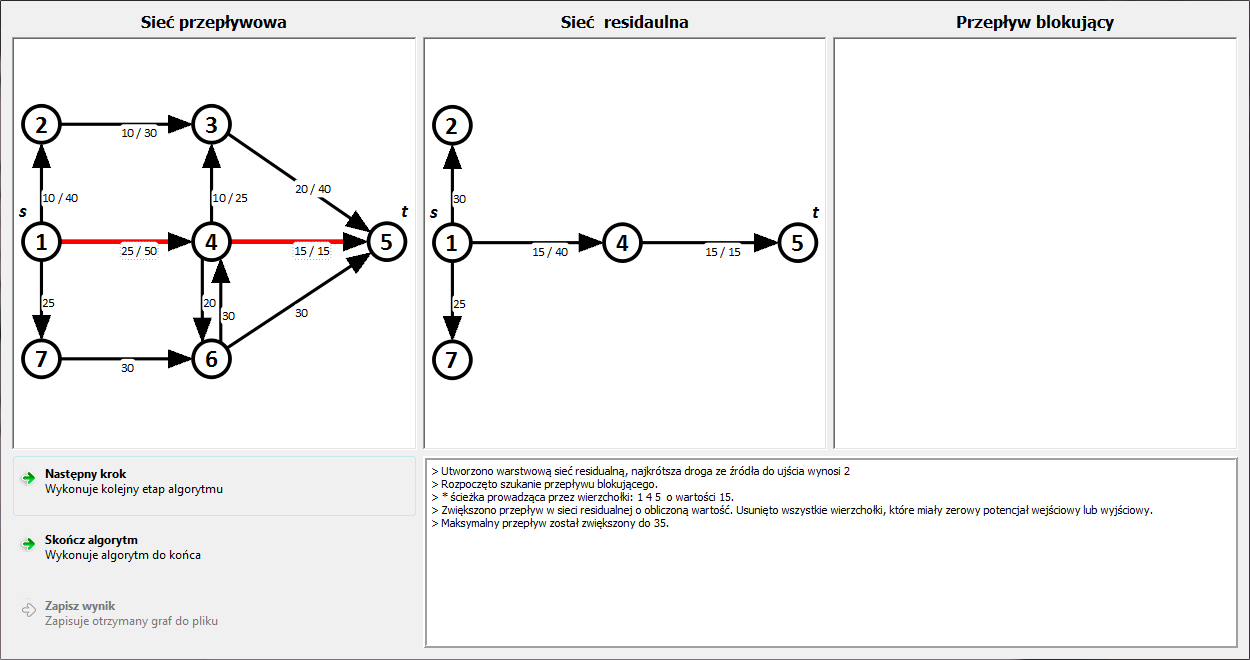
\includegraphics[width=0.9\linewidth]{./img/mkm04.jpg}
 		\end{subfigure}\par\bigskip
 		\begin{subfigure}{\textwidth}
 			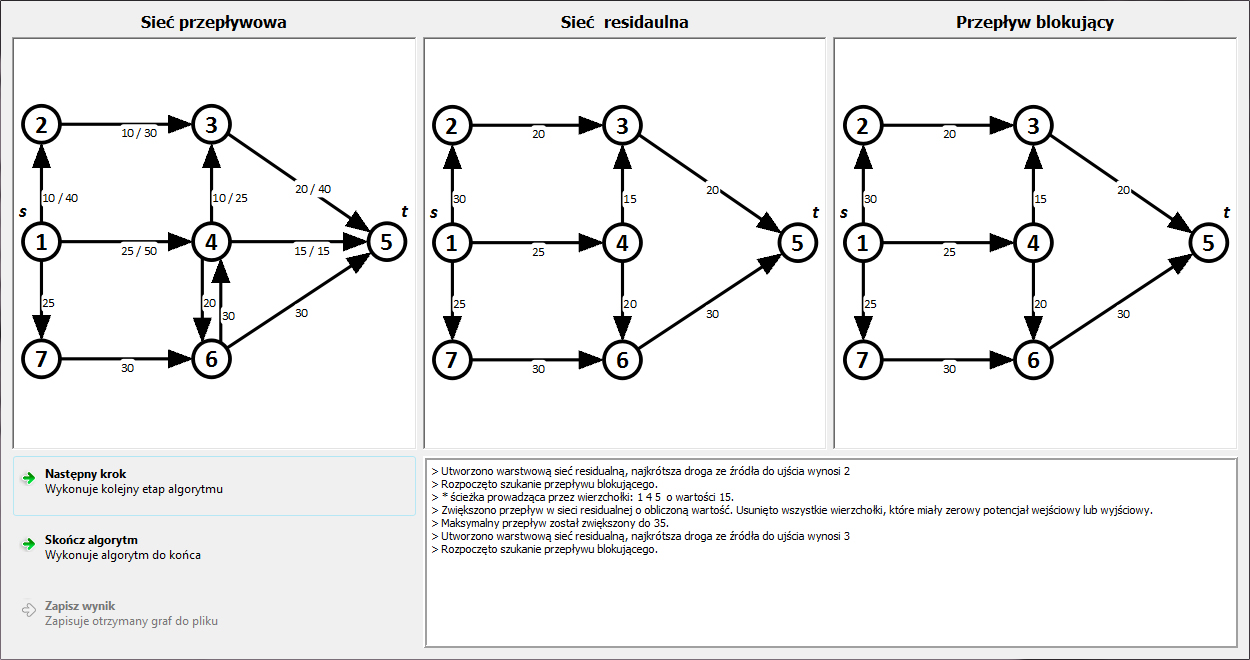
\includegraphics[width=0.9\linewidth]{./img/mkm05.jpg}
 		\end{subfigure}
 	\end{figure}
 	\begin{figure}
 		\ContinuedFloat
 		\begin{subfigure}{\textwidth}
 			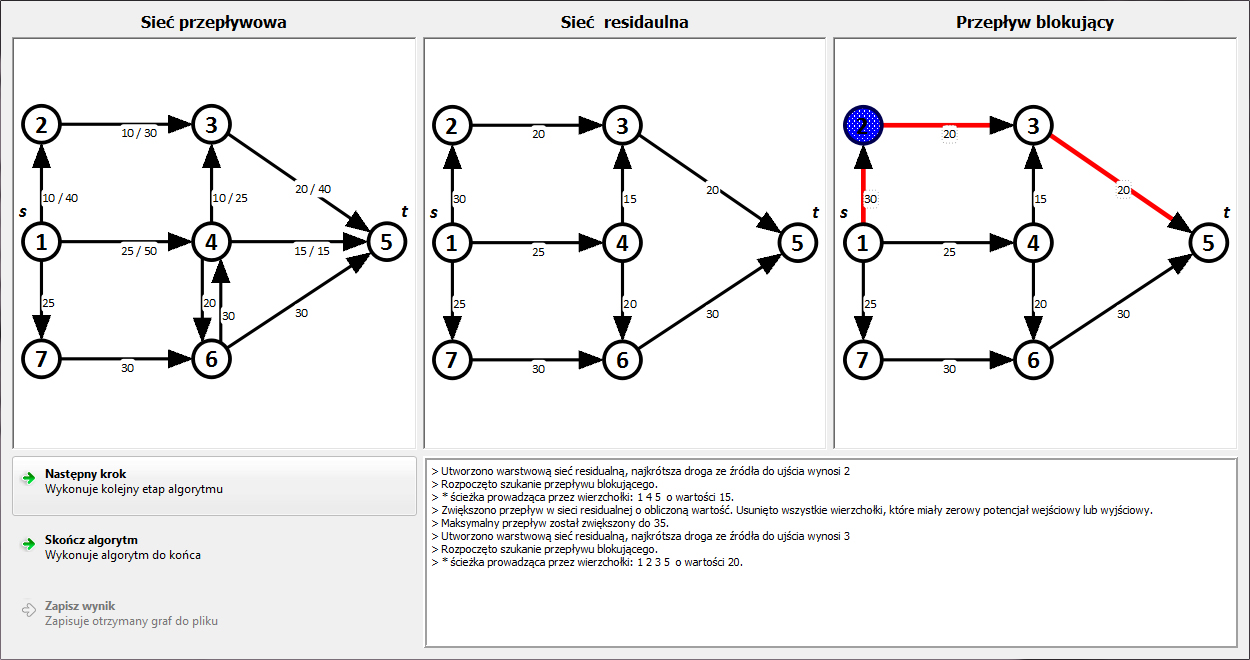
\includegraphics[width=0.9\linewidth]{./img/mkm06.jpg}
 		\end{subfigure}\par\bigskip
 		\begin{subfigure}{\textwidth}
 			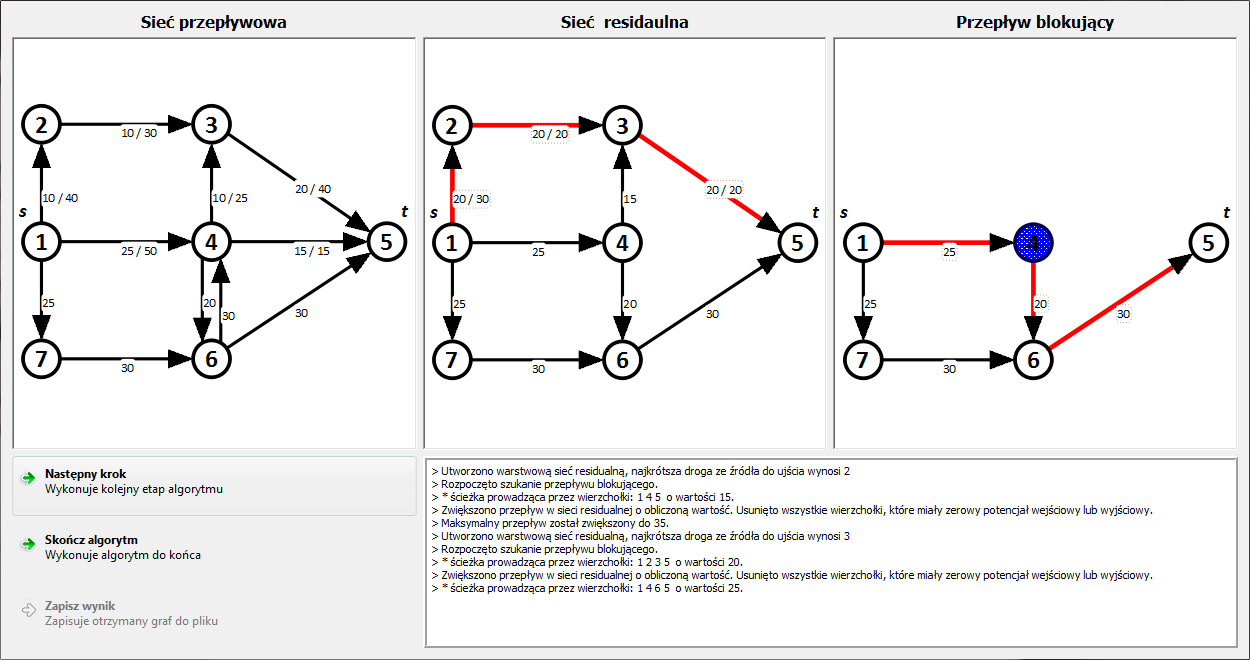
\includegraphics[width=0.9\linewidth]{./img/mkm08.jpg}
 		\end{subfigure}\par\bigskip
 		\begin{subfigure}{\textwidth}
 			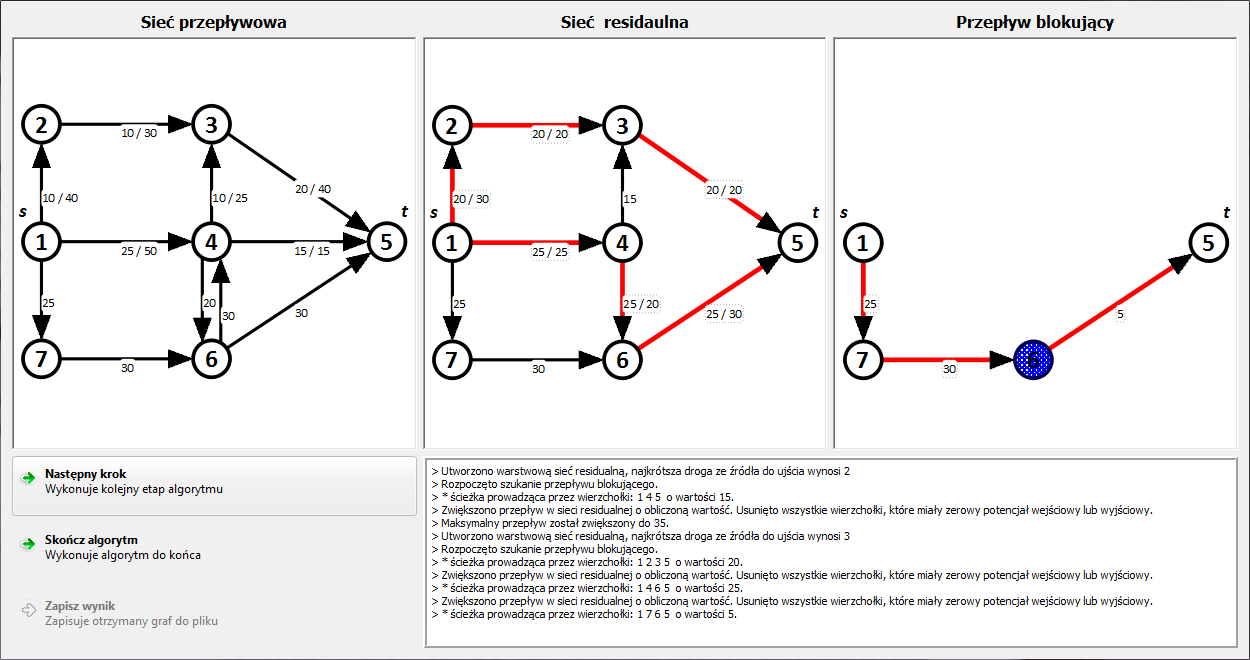
\includegraphics[width=0.9\linewidth]{./img/mkm10.jpg}
 		\end{subfigure}
 	\end{figure}
 	\begin{figure}
 		\ContinuedFloat
 		\begin{subfigure}{\textwidth}
 			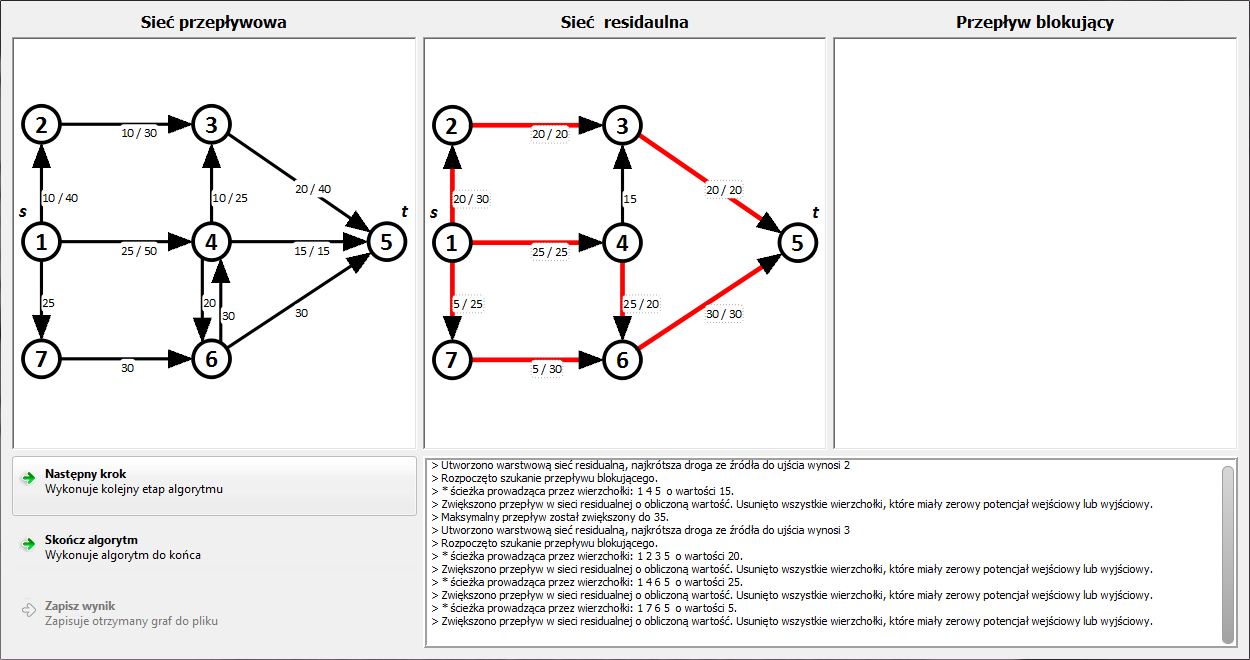
\includegraphics[width=0.9\linewidth]{./img/mkm11.jpg}
 		\end{subfigure}
 		\begin{subfigure}{\textwidth}
 			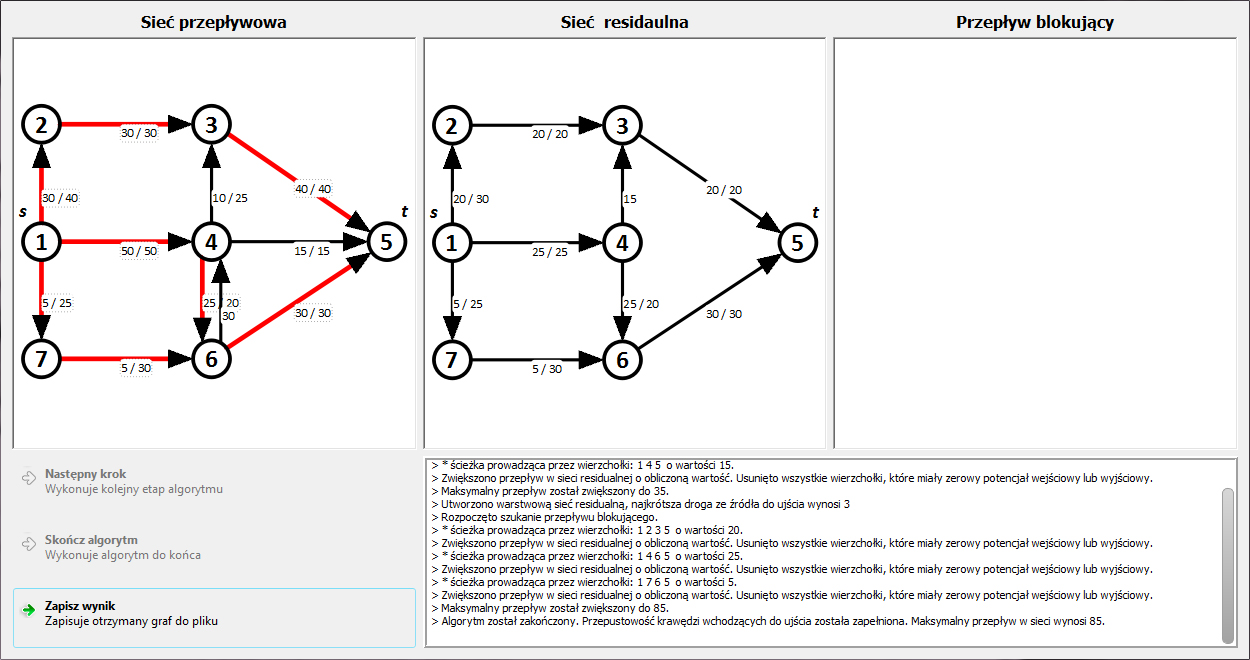
\includegraphics[width=0.9\linewidth]{./img/mkm12.jpg}
 		\end{subfigure}
 	\end{figure}
\end{appendices}